\chapter{State of the Art}\label{chap:state_art}

\section{Understanding the Basics}

\noindent Before diving into a detailed explanation, it is essential to understand some foundational concepts. The following sections provide simplified explanations of these key concepts:

\begin{enumerate}
    \item What is \ac{AR} ?
    \item What is lens distortion?
    \item What is the $R^3$ software?
\end{enumerate}

\subsection{What is augmented reality}

\noindent \ac{AR} is a technology that overlays digital information—such as images, sounds, or text—onto the real world. Unlike \ac{VR}, which creates a fully immersive digital environment, \ac{AR} enhances reality by adding interactive, computer-generated elements. For example, in mobile applications or games like Pokémon GO, digital characters appear as if they are part of the physical world when viewed through the device's camera.\ac{AR} is used in various fields, including gaming, retail, education, and training, to enrich the user experience with additional layers of digital content.

\noindent wTVision implements \ac{AR} on video streaming platforms. Figures \ref{fig:AG_4} and \ref{fig:AG4_overlay} show a frame from a video of an \ac{AR} scene developed by wTVision.

\begin{figure}[h]
    \centering
    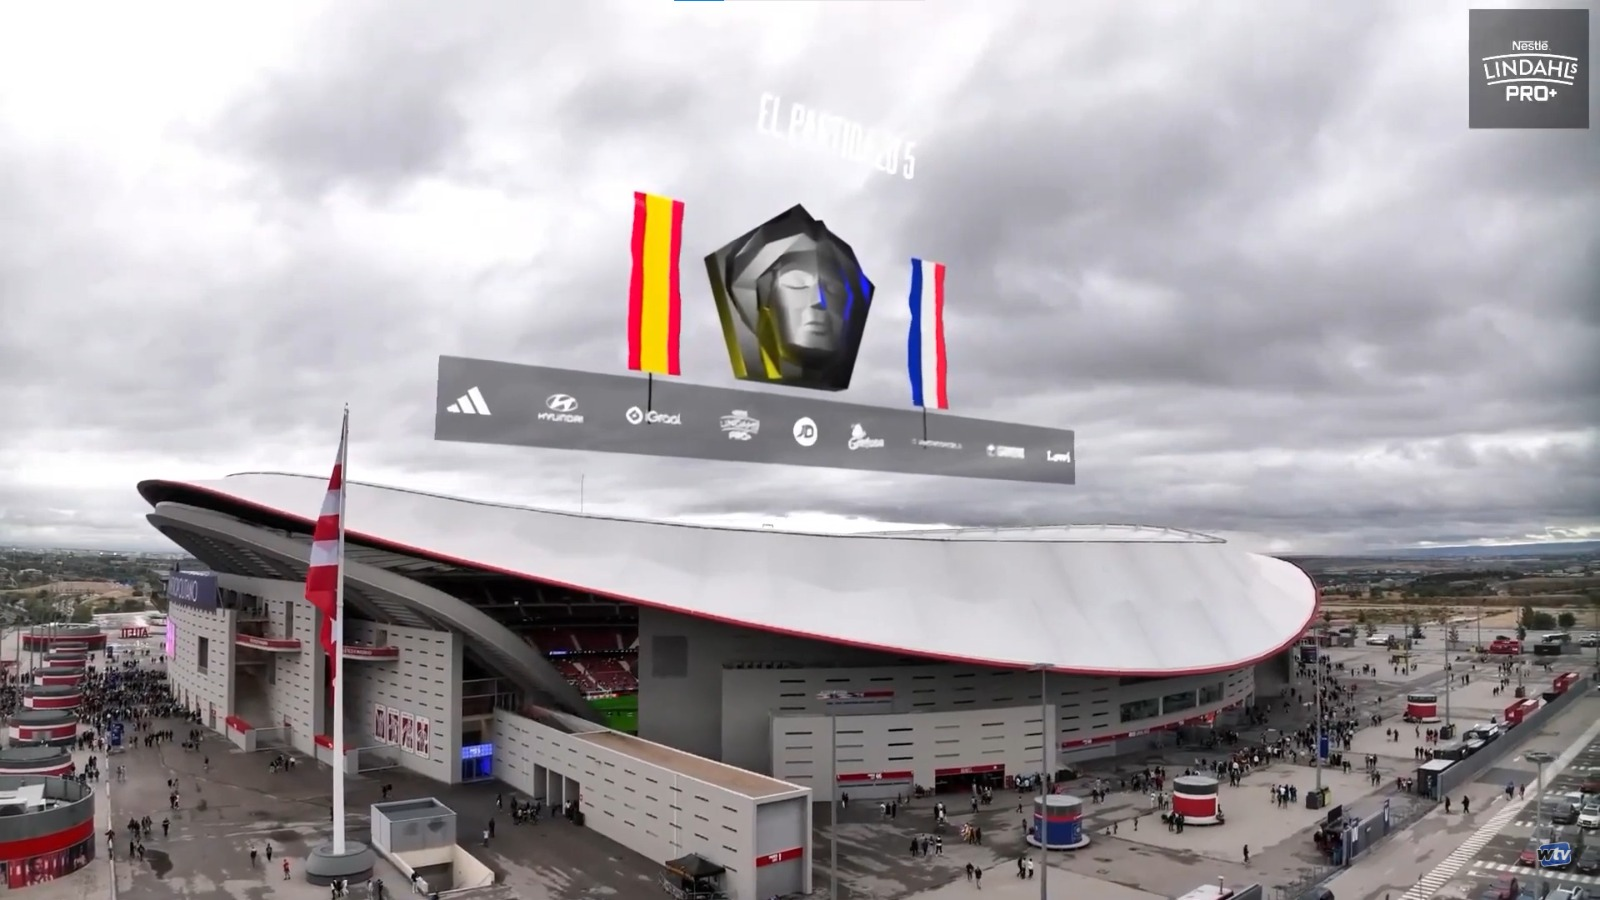
\includegraphics[width=\textwidth]{Images/02stateart/AG_4.jpeg}
    \caption{Example of an \ac{AR} scene developed by wTVision}
    \label{fig:AG_4}
\end{figure}

\begin{figure}[h]
    \centering
    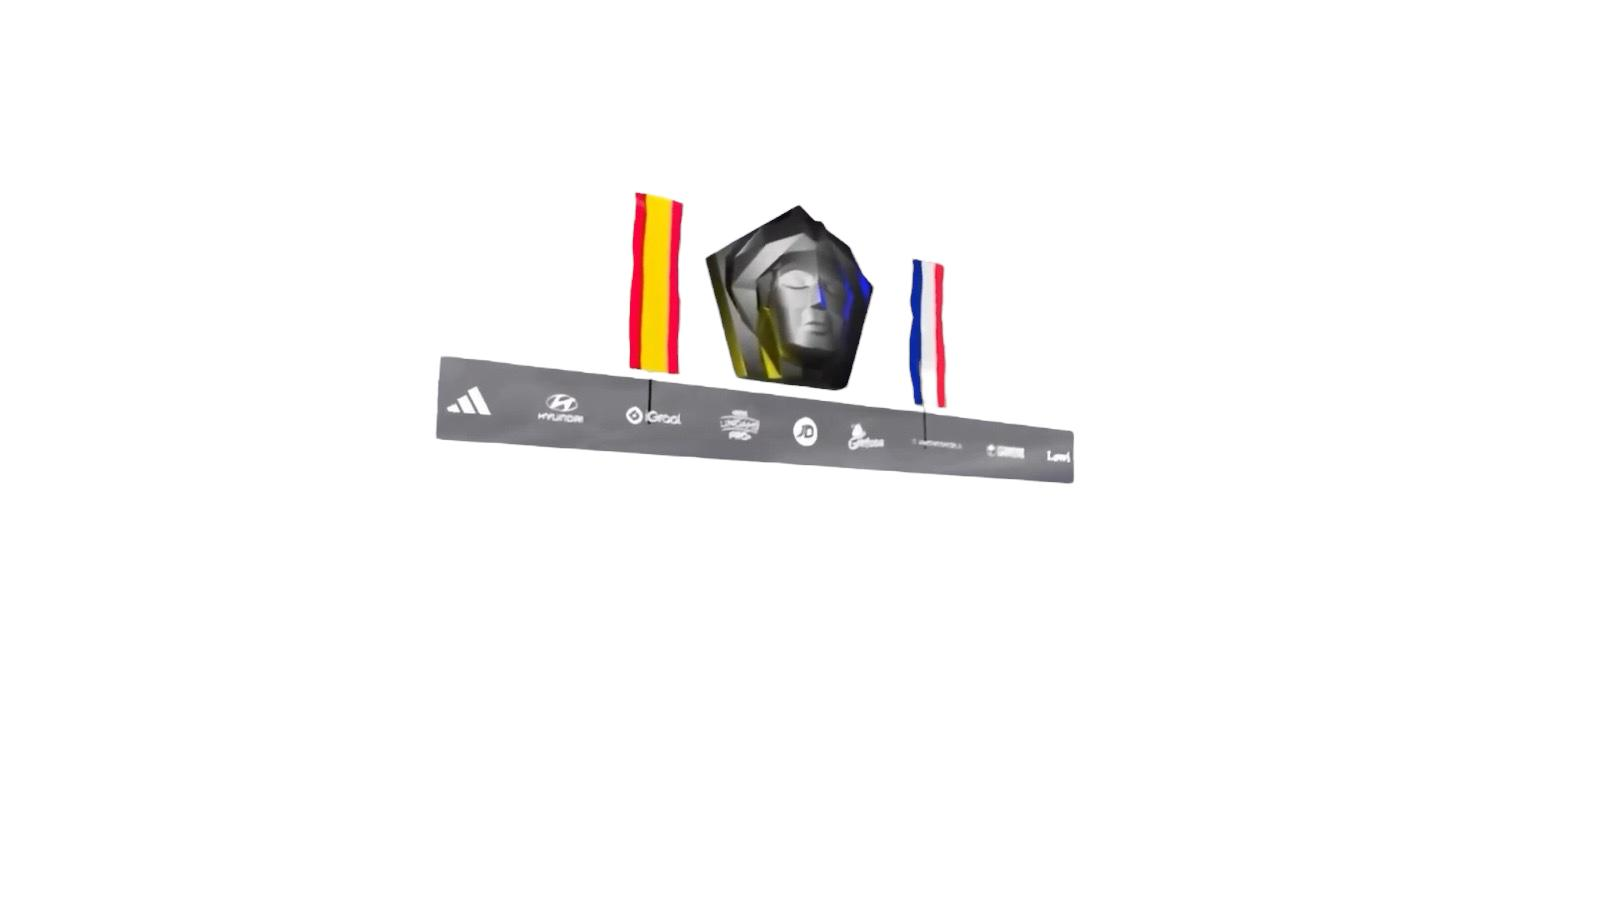
\includegraphics[width=\textwidth]{Images/02stateart/AG_4_overlay.jpeg}
    \caption{Overlay used in the scene shown in Figure \ref{fig:AG_4}}
    \label{fig:AG4_overlay}
\end{figure}

\subsection{What is Lens Distortion}

\noindent Lens distortion is an optical effect in which straight lines appear curved or warped in a photograph, image, or video due to imperfections in the lens shape and due to the physics of optics. This effect commonly occurs with wide-angle and zoom lenses, distorting the real-world perspective and causing objects near the edges of the image to appear stretched or compressed. Figure \ref{fig:lens} illustrates various types of lens distortion.

\begin{figure}[h]
    \centering
    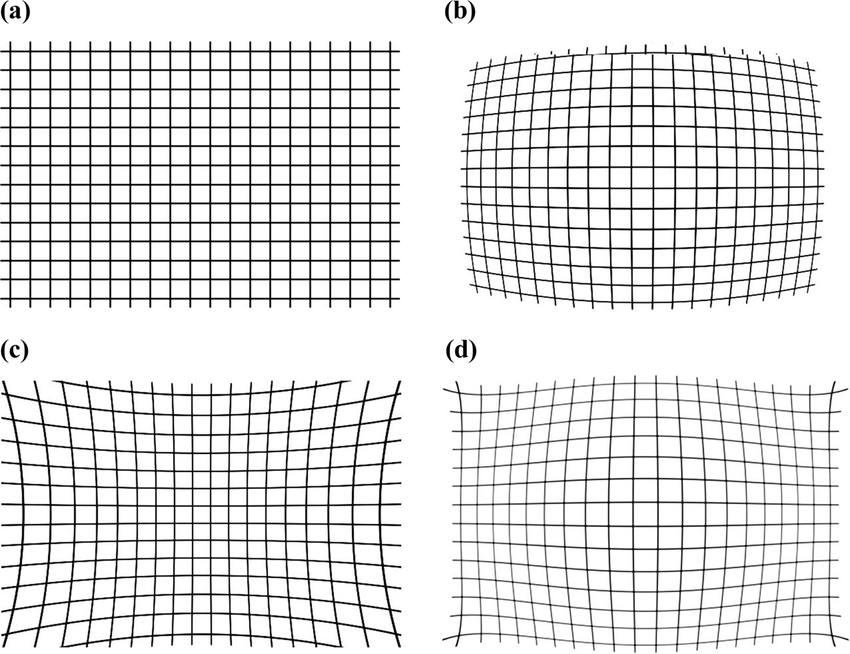
\includegraphics[width=\textwidth]{Images/02stateart/Types-of-lens-distortion-a-Non-distortion-b-Barrel-distortion-c-Pincushion.tif.png}
    \caption{Types of lens distortions: (a) Non-distortion, (b) Barrel distortion, (c) Pincushion distortion, (d) Mixed types of distortion}
    \label{fig:lens}
\end{figure}

\noindent Cameras used by wTVision have some degree of distortion, although it is not very noticeable. However, when inserting virtual overlays in a video, it is crucial to distort the virtual environment in the same way the camera lens distorts the real world. This ensures that virtual objects appear realistic and correctly aligned. Without this distortion, virtual objects would appear out of place when inserted into the real-world scene.

\subsection{What is the $R^3$ Software}

\noindent To address this issue, wTVision developed the $R^3$ software. This tool includes an engine and a software platform that provides the necessary technology to create and render digital environments. Within the platform, the "Space Designer" tool allows developers to build, layout, and arrange the virtual environment where the interactive experience takes place. While the engine handles rendering graphics, processing physics, and managing assets, the Space Designer offers an interactive, visual interface for creating the look and feel of the virtual world. Figure \ref{fig:interface} shows the $R^3$ Space Designer interface.

\begin{figure}[h]
    \centering
    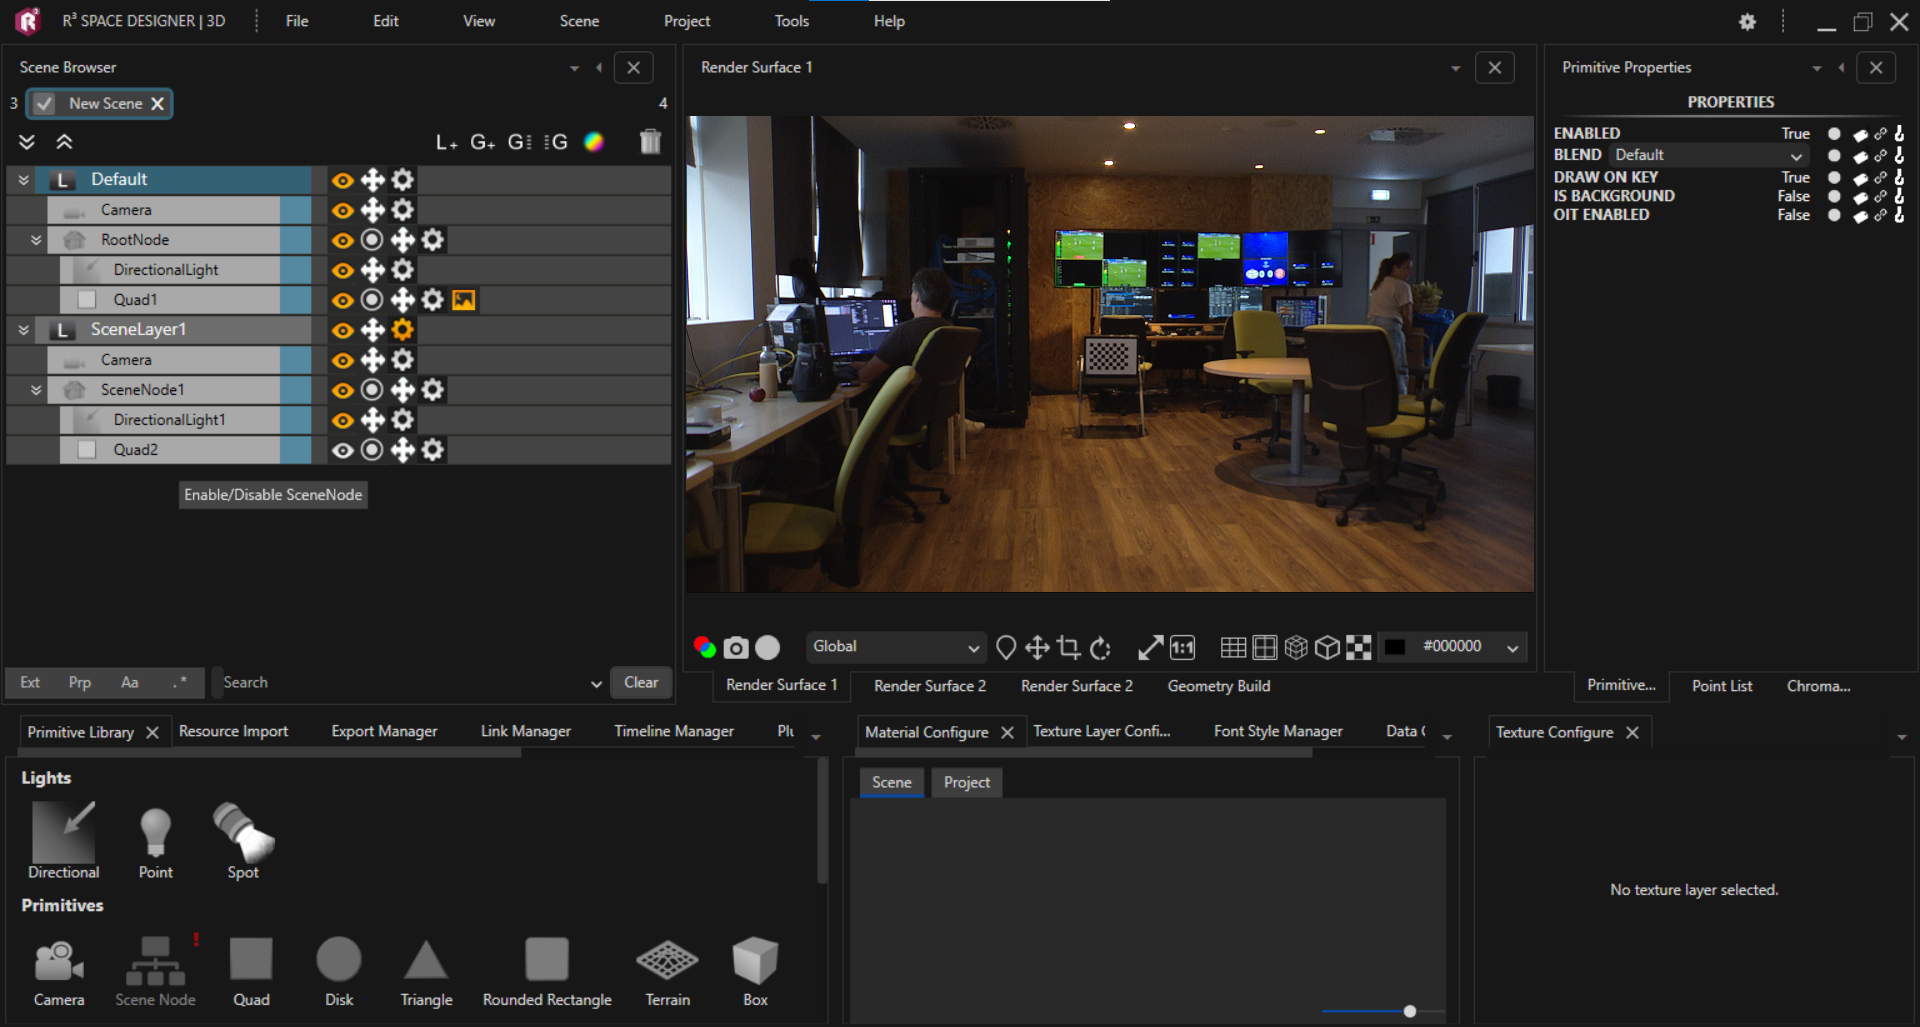
\includegraphics[width=\textwidth]{Images/02stateart/interface.png}
    \caption{$R^3$ Space Designer interface}
    \label{fig:interface}
\end{figure}

\section{Virtual Environment Calibration}

\noindent Earlier, we mentioned that wTVision developed the $R^3$ software to calibrate the virtual environment. This section explains why they developed a specialized tool instead of using existing tools like OpenCV for determining rectification coefficients, and it examines the pros and cons of the software.

\subsection{Common Lens Distortion Problems}

\noindent First, let’s clarify how typical lens distortion issues are handled. For example, photographers using professional cameras frequently encounter distorted images, as shown in Figure \ref{fig:prof_camera}.

\begin{figure}[h]
    \centering
    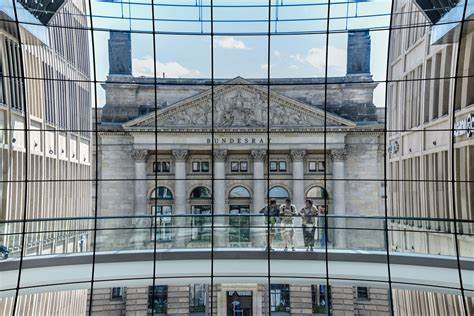
\includegraphics[width=\textwidth]{Images/02stateart/professional camera.png}
    \caption{Example of a distorted image taken with a professional camera}
    \label{fig:prof_camera}
\end{figure}

\noindent To correct these distortions, the OpenCV library is often used by applying specific distortion coefficients.

\noindent The main types of lens distortion are \textbf{Radial Distortion} and \textbf{Tangential Distortion}. Each type has distinct causes and visual effects, which are explained below.

\subsection{Types of Lens Distortion}

\begin{itemize}
    \item \textbf{Radial Distortion:}
    
    Radial distortion occurs when light rays bend unevenly as they pass through the lens, causing straight lines to appear curved. This distortion is more pronounced at the image edges and is mathematically described by:

    \begin{align}
        x_{\text{distorted}} &= x \left(1 + k_1 r^2 + k_2 r^4 + k_3 r^6\right) \\
        y_{\text{distorted}} &= y \left(1 + k_1 r^2 + k_2 r^4 + k_3 r^6\right)
    \end{align}

    where \( k_1 \), \( k_2 \), and \( k_3 \) are radial distortion coefficients, and \( r \) represents the distance from the optical center.

    \item \textbf{Tangential Distortion:}
    
    Tangential distortion results from misalignment between the camera sensor and the lens, causing image points to shift in a direction based on their position. This distortion is modeled by:

    \begin{align}
        x_{\text{distorted}} &= x + \left[2 p_1 x y + p_2 \left(r^2 + 2 x^2\right)\right] \\
        y_{\text{distorted}} &= y + \left[p_1 \left(r^2 + 2 y^2\right) + 2 p_2 x y\right]
    \end{align}

    where \( p_1 \) and \( p_2 \) are tangential distortion coefficients.
\end{itemize}

\subsection{Correcting Lens Distortion with OpenCV}

\noindent To correct these distortions, OpenCV uses a set of distortion coefficients. The five main coefficients—\( k_1 \), \( k_2 \), \( p_1 \), \( p_2 \), and \( k_3 \)—capture both radial and tangential distortion effects:

\begin{equation}
    \text{Distortion Coefficients} = \left(\begin{array}{lllll}
        k_1 & k_2 & p_1 & p_2 & k_3
    \end{array}\right)
\end{equation}

\noindent OpenCV can use these coefficients to rectify distorted images.

\subsection{Challenges in Using OpenCV for Virtual Environment Calibration}

\noindent As mentioned, this project does not aim to rectify images but to calibrate the geometry of a virtual environment. For this, we need to determine the camera's distortion coefficients.

\noindent OpenCV calculates distortion coefficients like \( k_1 \), \( k_2 \), \( p_1 \), \( p_2 \), and \( k_3 \) to correct image distortion. However, for our specific needs, additional coefficients are required that OpenCV cannot provide:

\begin{itemize}
    \item \textbf{Central-Shift:} Due to misaligned lenses, the real-world origin point (0,0,0) and the virtual one may differ, necessitating a central-shift coefficient.
    \item \textbf{No Parallax Effect Coefficient:} To achieve the No Parallax Effect, the virtual environment must behave similarly to the camera, with minimized parallax. The No Parallax Effect coefficient aims to eliminate the apparent shift in object positions due to a viewpoint change. Figure \ref{fig:pen} illustrates this phenomenon. The first image depicts a person's view with both eyes open, offering a complete perspective of the object. In contrast, the second image illustrates the shift in perspective that occurs when one eye is closed, significantly altering the perception of the object.
    \item \textbf{Field of View (FoV):} The \textbf{field of view (FOV)} is the extent of the scene captured by the camera, measured in degrees. It depends on the focal length and sensor size, with wider angles covering more of the scene and narrower angles focusing on a smaller area. Adjusting the camera's zoom changes the FoV, alters the perceived distance of objects. Replicating this effect in \ac{AR} requires altering the FoV in the virtual environment.
\end{itemize}


\begin{figure}
    \centering
    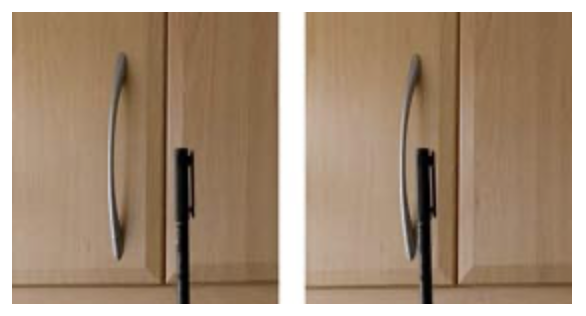
\includegraphics[width=\textwidth]{Images/02stateart/pen.png}
    \caption{Parallax Effect with the human eye.Left picture depicts
    a person’s view with both eyes open. Right picture depicts the shift in perspective that occurs when one eye is closed.}
    \label{fig:pen}
\end{figure}

\section{Communication Between Python and \texorpdfstring{$R^3$}{R3}}
\label{sec:communication_python_r3}

\noindent In this work, the communication between Python and the \textit{R\textsuperscript{3}} software is implemented using sockets. Sockets are a fundamental mechanism in computer systems that enable processes to exchange data. While traditionally used for communication over a network, sockets can also be employed to facilitate communication between processes on the same machine, leveraging the system's networking stack for local inter-process communication (IPC) \cite{stevens2003unix, silberschatz2018os}.

\subsection{Why Sockets for Communication}
\noindent Sockets provide a simple and robust interface for connecting applications written in different programming languages. In this case, Python acts as the controlling script, orchestrating the execution of the \textit{R\textsuperscript{3}} software. Using sockets offers the following advantages:
\begin{itemize}
    \item \textbf{Language Agnosticism:} Python and \textit{R\textsuperscript{3}} operate independently, and sockets enable communication without requiring language-specific bindings or modifications to the software \cite{beejGuide, pythonDocsSocket}.
    \item \textbf{Asynchronous Communication:} Sockets allow Python to send commands to \textit{R\textsuperscript{3}} and wait to receive responses at different rates, enabling efficient two-way communication \cite{stevens2003unix}.
    \item \textbf{Local Communication:} Although sockets are often associated with network communication, they can be used for local IPC by binding the socket to the loopback interface (localhost). This ensures that all communication remains within the same machine, minimizing latency and security concerns \cite{silberschatz2018os}.
\end{itemize}

\subsection{Implementation Overview}
\noindent The implementation of the communication relies on a server-client model \cite{beejGuide}:
\begin{enumerate}
    \item \textbf{Socket Initialization:} A socket initialized in Python connection it to the $R^3$ software, configured as the server, and bound to a specific port (9009) on the loopback address (127.0.0.1) \cite{pythonDocsSocket}.
    \item \textbf{Connection from \textit{R\textsuperscript{3}}:} Python acts as a client, connecting to $R^3$.
    \item \textbf{Message Exchange:} Once connected, Python sends commands or data to \textit{R\textsuperscript{3}}, and the latter processes the instructions and responds via the same socket \cite{stevens2003unix}.
    \item \textbf{Closing the Connection:} After the data exchange is complete, the connection is gracefully closed, releasing resources.
\end{enumerate}

\subsection{Commands for Interaction with the Engine}
\label{subsec:engine_commands}

\noindent The communication between Python and the \textit{R\textsuperscript{3}} software, as outlined in Section~\ref{sec:communication_python_r3}, enables the execution of specific commands to interact with the engine's functionality. Below, we describe the key commands used in this implementation, their purposes, and their syntax, as demonstrated in the provided examples.

\subsubsection{Basic Engine Interaction Commands}
\begin{itemize}
    \item \textbf{TakeSnapshot:} This command captures a snapshot of the render surface and saves it as a PNG image. The default save location is the "Projects" folder, but users can specify a custom path and filename. The command supports two syntaxes:
    \begin{itemize}
        \item \texttt{engine.takeSnapshot "file\_name"}: Saves the snapshot with the specified filename in the default "Projects" folder.
        \item \texttt{engine.takeSnapshot "path\_with\_filename"}: Saves the snapshot at the specified path with the given filename.
    \end{itemize}
    Upon success, the engine responds with \texttt{"OK: SNAPSHOT TAKEN"}. If an invalid path is provided, it returns an error message: \texttt{"ERROR: SNAPSHOT - INVALID PATH"}. For example:
    \begin{verbatim}
    engine.takeSnapshot "JornalNoiteTicker"
    \end{verbatim}
    saves a snapshot named "JornalNoiteTicker.png" in the default location, while:
    \begin{verbatim}
    engine.takeSnapshot "C:/Users/john.doe/Desktop/JornalNoiteTicker"
    \end{verbatim}
    saves it to a specific desktop path.

    \item \textbf{GetSnapshot:} This command retrieves a snapshot previously taken with \texttt{TakeSnapshot} and returns it as a base64-encoded string. It is essential to use \texttt{TakeSnapshot} before invoking \texttt{GetSnapshot}, as the latter relies on the existence of a snapshot file. The command supports two syntaxes:
    \begin{itemize}
        \item \texttt{engine.getSnapshot "file\_name"}: Retrieves the snapshot with the specified filename from the default "Projects" folder.
        \item \texttt{engine.getSnapshot "path\_with\_filename"}: Retrieves the snapshot from the specified path and filename.
    \end{itemize}
    Upon success, the engine responds with:
    \begin{verbatim}
    "OK: <IMAGE> base64string <IMAGE>"
    \end{verbatim}
    If the snapshot file cannot be found or the path is invalid, it returns an error message, such as:
    \begin{verbatim}
    "ERROR: GETSNAPSHOT - COULD NOT READ LAST SNAPSHOT FILE"
    "ERROR: GETSNAPSHOT - INVALID PATH"
    \end{verbatim}
    For instance:
    \begin{verbatim}
    engine.getSnapshot "JornalNoiteTicker"
    \end{verbatim}
    returns the base64-encoded image data for the snapshot named "JornalNoiteTicker.png" in the default location.

    \item \textbf{Get:} This command retrieves the current tracking packet from a specified tracking camera, providing detailed camera parameters and status. The syntax is:
    \begin{verbatim}
    engine.tracking "tracking_camera_name" get
    \end{verbatim}
    Upon success, the engine responds with:
    \begin{verbatim}
    "OK: CURRENT CAMERA PARAMETERS:"
    \end{verbatim}
    followed by a JSON-like structure containing parameters such as field of view (FovX, FovY), aspect ratio, position (PosX, PosY, PosZ), rotation (RotX, RotY, RotZ), and other metadata like view matrix, center coordinates, and sensor size. For example:
    \begin{verbatim}
    engine.tracking "Cam0" get
    \end{verbatim}
    might return a response detailing the parameters of the "Cam0" tracking camera, including:
    \begin{verbatim}
    "FovX": 80.0, "FovY": 50.0, ...
    \end{verbatim}
\end{itemize}

\subsubsection{Scene Export Commands}
\noindent In addition to the basic engine interaction commands, the system supports a set of more complex \textit{Scene Export} commands for managing and manipulating scene properties within \textit{R\textsuperscript{3}}. These commands operate on export entities (e.g., properties like transform positions, scales, or text values) and can be executed individually or in batches (via \textit{MultiExport}). Below, we detail each command and its functionality:

\begin{itemize}
    \item \textbf{SetValue:} This command sets the value of a specific export property within a scene. The syntax is:
    \begin{verbatim}
    scene "project_ref/scene_ref" export "export_name" SetValue "value"
    \end{verbatim}
    \item \textbf{Rename:} This command renames an existing export within a scene. The syntax is:
    \begin{verbatim}
    scene "project_ref/scene_ref" export "export_name" rename "new_name"
    \end{verbatim}
    \item \textbf{GetValue:} This command retrieves the current value of a specific export property within a scene. The syntax is:
    \begin{verbatim}
    scene "project_ref/scene_ref" export "export_name" getValue
    \end{verbatim}
    \item \textbf{MultiExport Commands:} These commands allow batch operations on multiple exports. Example:
    \begin{verbatim}
    scene "JornalNoite/teste" export "transform.scale" SetValue "1,2,1"
          "text" SetValue "player_name" "alpha" SetValue "0.5"
    \end{verbatim}
    returns:
    \begin{verbatim}
    "OK: SCENE EXPORT SETVALUE - Value Set."
    "OK: SCENE EXPORT SETVALUE - Value Set."
    "OK: SCENE EXPORT SETVALUE - Value Set."
    \end{verbatim}
\end{itemize}

\noindent These \textit{Scene Export} commands provide fine-grained control and automation through Python scripts, enabling efficient real-time scene manipulation.


\subsection{Benefits of Local Socket Communication}
\noindent By utilizing sockets for communication between Python and \textit{R\textsuperscript{3}}, this setup ensures modularity and scalability. Python and \textit{R\textsuperscript{3}} remain decoupled, allowing for independent updates or replacements of either component without affecting the communication protocol. Additionally, the use of the loopback interface ensures that no external networking hardware or configuration is required \cite{silberschatz2018os}.

\subsection{Applications and Future Potential}
\noindent This socket-based architecture facilitates a variety of use cases, such as:
\begin{itemize}
    \item Automating tasks in \textit{R\textsuperscript{3}} through Python scripts.
    \item Integrating Python's data analysis and visualization capabilities with \textit{R\textsuperscript{3}}'s functionality.
    \item Enabling real-time monitoring and feedback loops between Python and \textit{R\textsuperscript{3}}.
\end{itemize}

\noindent In summary, the use of sockets for communication between Python and \textit{R\textsuperscript{3}} provides a flexible and efficient solution for inter-process communication, paving the first step to automate the lens calibration.



